\PassOptionsToPackage{unicode=true}{hyperref} % options for packages loaded elsewhere
\PassOptionsToPackage{hyphens}{url}
%
\documentclass[]{article}
\usepackage{lmodern}
\usepackage{amssymb,amsmath}
\usepackage{ifxetex,ifluatex}
\usepackage{fixltx2e} % provides \textsubscript
\ifnum 0\ifxetex 1\fi\ifluatex 1\fi=0 % if pdftex
  \usepackage[T1]{fontenc}
  \usepackage[utf8]{inputenc}
  \usepackage{textcomp} % provides euro and other symbols
\else % if luatex or xelatex
  \usepackage{unicode-math}
  \defaultfontfeatures{Ligatures=TeX,Scale=MatchLowercase}
\fi
% use upquote if available, for straight quotes in verbatim environments
\IfFileExists{upquote.sty}{\usepackage{upquote}}{}
% use microtype if available
\IfFileExists{microtype.sty}{%
\usepackage[]{microtype}
\UseMicrotypeSet[protrusion]{basicmath} % disable protrusion for tt fonts
}{}
\IfFileExists{parskip.sty}{%
\usepackage{parskip}
}{% else
\setlength{\parindent}{0pt}
\setlength{\parskip}{6pt plus 2pt minus 1pt}
}
\usepackage{hyperref}
\hypersetup{
            pdftitle={Supplementary Material (SM)},
            pdfborder={0 0 0},
            breaklinks=true}
\urlstyle{same}  % don't use monospace font for urls
\usepackage[margin=1in]{geometry}
\usepackage{graphicx,grffile}
\makeatletter
\def\maxwidth{\ifdim\Gin@nat@width>\linewidth\linewidth\else\Gin@nat@width\fi}
\def\maxheight{\ifdim\Gin@nat@height>\textheight\textheight\else\Gin@nat@height\fi}
\makeatother
% Scale images if necessary, so that they will not overflow the page
% margins by default, and it is still possible to overwrite the defaults
% using explicit options in \includegraphics[width, height, ...]{}
\setkeys{Gin}{width=\maxwidth,height=\maxheight,keepaspectratio}
\setlength{\emergencystretch}{3em}  % prevent overfull lines
\providecommand{\tightlist}{%
  \setlength{\itemsep}{0pt}\setlength{\parskip}{0pt}}
\setcounter{secnumdepth}{5}
% Redefines (sub)paragraphs to behave more like sections
\ifx\paragraph\undefined\else
\let\oldparagraph\paragraph
\renewcommand{\paragraph}[1]{\oldparagraph{#1}\mbox{}}
\fi
\ifx\subparagraph\undefined\else
\let\oldsubparagraph\subparagraph
\renewcommand{\subparagraph}[1]{\oldsubparagraph{#1}\mbox{}}
\fi

% set default figure placement to htbp
\makeatletter
\def\fps@figure{htbp}
\makeatother

\usepackage{xr}
\usepackage{mathtools}
\usepackage{mathrsfs}
\usepackage{hyperref}
\usepackage[left]{lineno}
\usepackage{amsmath}
\linenumbers
\externaldocument{Current-Version}
\usepackage{float}
\usepackage{flafter}

\title{Supplementary Material (SM)}
\author{}
\date{\vspace{-2.5em}}

\begin{document}
\maketitle

Throughout this supplement, we set use dot notation for time derivatives
so that \(\dot f(x,t)=\frac{\partial }{\partial t}f(x,t)\) and set
\(\Delta=\sum_{i=1}^d\frac{\partial^2}{\partial x_i^2}\) the Laplace
operator on \(\mathbb{R}^d\), except in \S\ref{caC} where \(\Delta\)
represents a random variable.

\hypertarget{sufficient-conditions-for-finite-mean-variance-and-total-abundance-in-the-deterministic-case}{%
\section{\texorpdfstring{Sufficient conditions for finite mean, variance
and total abundance in the deterministic case
\label{finite}}{Sufficient conditions for finite mean, variance and total abundance in the deterministic case }}\label{sufficient-conditions-for-finite-mean-variance-and-total-abundance-in-the-deterministic-case}}

Recall that \(m(\nu,x)\) is shorthand for \(m\big((K\nu)(x,t),x\big)\).
That is, \(m:[0,+\infty)\times\mathbb{R}\to\mathbb{R}\). Following our
assumptions of the main text, we have that \(m(h,x)\) is differentiable
with respect to both \(x\) and \(h\) and there exists \(r\in\mathbb{R}\)
such that \(m(h,x)\leq r\) across all \(h\geq0\) and \(x\in\mathbb{R}\).
As in the main text, we also assume the initial condition \(u(x)\) is
continuous and integrable in \(x\) and satisfies \begin{equation}
0\leq\int_{\mathbb{R}}(|x|+x^2)u(x)dx<+\infty
\end{equation} and consider the Cauchy problem
\begin{equation}\label{PDE_SM}
\left\{\begin{matrix}
\dot\nu(x,t)=m(\nu,x)\nu(x,t)+\frac{\mu}{2}\Delta\nu(x,t) & t>0\\
\nu(x,0)=u(x) & t=0.
\end{matrix}\right.
\end{equation}

According to Theorem 2.5.6 of Zheng (2004), if the operator \(F\)
defined by \(\nu(x,t)\to m(\nu,x)\nu(x,t)\) is locally Lipschitz,
corresponding to equation (\ref{local_lipschitz}) of the main text, then
for some maximal \(T>0\) problem (\ref{PDE_SM}) admits a unique local
classical solution \(\nu(x,t)\) for \(t\in[0,T)\). Furthermore, either
\(T=+\infty\) or \(T<+\infty\) and
\(\lim_{t\uparrow T}\int_\mathbb{R}|\nu(x,t)|dx=+\infty\). In this
section we show that our assumption \(m(h,x)\leq r\) for all \(h\geq0\)
and \(x\in\mathbb{R}\) implies \(T=+\infty\). Replacing \(m\) with it's
upper bound \(r\in\mathbb{R}\), equation (\ref{PDE_SM}) reduces to a
simple parabolic equation that can be solved using elementary techniques
(Farlow 1993). In particular, when \(m(\nu,x)\equiv0\) denote the
solution to (\ref{PDE_SM}) by \(\nu_0(x,t)\). Then, denoting
\begin{equation}
\Phi(x,t)=\frac{\exp\left(-x^2/2\mu t\right)}{\sqrt{2\pi\mu t}},
\end{equation} we have \begin{equation}
\nu_0(x,t)=\int_{\mathbb{R}}\Phi(x-y,t)\nu(y,0)dy.
\end{equation} In the more general case, when
\(m(\nu,x)\equiv r\in\mathbb{R}\), equation (\ref{PDE_SM}) has the
solution \(\nu_r(x,t)=e^{rt}\nu_0(x,t)\). Hence, \(\nu_r(x,t)\geq0\) for
all \(x\in\mathbb{R}\) and
\(\int_\mathbb{R}\nu_r(x,t)dx=e^{rt}N(0)<+\infty\) for all \(t\geq0\).
Furthermore, denoting \begin{equation}
\begin{matrix}
N_r(t)&=&\int_\mathbb{R}\nu_r(x,t)dx, \\
p_r(x,t)&=&\nu_r(x,t)/N_r(t), \\
\bar x_r(t)&=&\int_\mathbb{R}xp_r(x,t)dx, \\
\sigma^2_r(t)&=&\int_\mathbb{R}(x-\bar x_r(t))^2p_r(x,t)dx, 
\end{matrix}
\end{equation} we have \begin{equation}
\bar x_r(t)=\int_\mathbb{R}x\int_\mathbb{R}\Phi(x-y,t)p(y,0)dydx=\int_\mathbb{R}yp(y,0)dy=\bar x(0),
\end{equation} \begin{equation}
\sigma_r^2(t)=\int_\mathbb{R}(x-\bar x_r(t))^2\int_\mathbb{R}\Phi(x-y,t)p(y,0)dydx=\int_\mathbb{R}\Big((y-\bar x(0))^2+\mu t\Big)p(y,0)dy=\sigma^2(0)+\mu t.
\end{equation} Hence, \(|\bar x_r(t)|,\sigma_r^2(t)<+\infty\) for all
\(t\geq0\). For the sake of contradiction, suppose there exists
\(x\in\mathbb{R}\) and \(t\geq0\) such that \(\nu(x,t)>\nu_r(x,t)\).
Then \begin{equation}
\nu(x,t)-\nu(x,0)=\int_0^tm(\nu,x)\nu(x,s)+\frac{\mu}{2}\Delta\nu(x,s)ds>\int_0^tr\nu_r(x,s)+\frac{\mu}{2}\Delta\nu_r(x,s)ds=\nu_r(x,t)-\nu(x,0)
\end{equation} which implies there exists \(h\geq0\) and
\(x\in\mathbb{R}\) such that \(m(h,x)>r\). But this contradicts our
assumption \(m(h,x)\leq r\) for all \(h\geq0\) and \(x\in\mathbb{R}\).
So we have \(\nu(x,t)\leq\nu_r(x,t)\) for each \(x\in\mathbb{R}\) and
\(t\geq0\). This implies that
\(N(t)=\int_\mathbb{R}\nu(x,t)dx<+\infty\), \begin{equation}
0\leq\int_\mathbb{R}x^2\nu(x,t)dx\leq\int_\mathbb{R}x^2\nu_r(x,t)dx<+\infty
\end{equation} and in particular \begin{equation}
0\leq\sigma^2(t)+\bar x^2(t)=\frac{1}{N(t)}\int_\mathbb{R}x^2\nu(x,t)dx<+\infty
\end{equation} for each \(t\geq0\).

\hypertarget{equilibrium-moments-for-a-deterministic-population-experiencing-logistic-growth-and-stabilizing-selection}{%
\section{\texorpdfstring{Equilibrium moments for a deterministic
population experiencing logistic growth and stabilizing selection
\label{equilib}}{Equilibrium moments for a deterministic population experiencing logistic growth and stabilizing selection }}\label{equilibrium-moments-for-a-deterministic-population-experiencing-logistic-growth-and-stabilizing-selection}}

Here we set out to show, given the initial conditions
\(\nu(\cdot,0)\in L^1(\mathbb{R})\) such that
\(\bar x(0)\in\mathbb{R}\), \(\sigma^2(0)\in[0,+\infty)\) and
\(N(0)\in(0,+\infty)\), and given the growth rate
\begin{equation}\label{m_log_stab}
m(\nu,x)=r-\frac{a}{2}(\theta-x)^2-c\int_\mathbb{R}\nu(y,t)dy
\end{equation} such that \(\theta\in\mathbb{R}\), \(a,c,\mu>0\) and
\(r>\tfrac{1}{2}\sqrt{\mu a}\), we have the following stable equilibrium
\(N_\infty=\lim_{t\to\infty}N(t)=\tfrac{1}{c}(r-\tfrac{1}{2}\sqrt{a\mu})\),
\(\bar x_\infty=\lim_{t\to\infty}\bar x(t)=\theta\) and
\(\sigma^2_\infty=\lim_{t\to\infty}\sigma^2(t)=\sqrt{\tfrac{\mu}{a}}\).

The mean fitness can be calculated as \begin{equation}
\bar m(t)=r-\frac{a}{2}((\theta-\bar x(t))^2+\sigma^2(t))-cN(t).
\end{equation} Recalling the ODE derived for \(N(t)\), \begin{equation}
\frac{d}{dt}N(t)=\bar m(t)N(t)=(r-\frac{a}{2}((\theta-\bar x(t))^2+\sigma^2(t))-cN(t))N(t),
\end{equation} solving for equilibrium total abundance \(\hat N\)
amounts to setting \(\frac{d}{dt}N(t)=0\) and solving for \(N(t)\).
Ignoring the equilibrium \(N(t)=0\), this reduces to solving
\(\bar m(t)=0\) for \(N(t)\), which returns \begin{equation}
\hat N=\frac{1}{c}\left(r-\frac{a}{2}\left((\theta-\hat{\bar x})^2-\hat\sigma^2\right)\right).
\end{equation} Unfortunately, deriving ODE for \(\bar x(t)\) and
\(\sigma^2(t)\) leads to expressions involving higher moments and
finding ODE for these higher moments will lead to expressions involving
yet even higher moments. To avoid this infinite regression, we find the
equilibrium abundance density \(\hat\nu(x)\) by solving
\(\frac{\partial}{\partial t}\nu(x,t)=0\) for \(\nu(x,t)\). This implies
the following ordinary differential equation \begin{equation}
\frac{d^2}{dx^2}\hat\nu(x)=\left(\frac{2c}{\mu}\hat N+\frac{a}{\mu}(\theta-x)^2-\frac{2r}{\mu}\right)\hat\nu(x)
\end{equation} which has the solution \begin{equation}
\hat\nu(x)=\frac{\hat N}{\sqrt{2\pi}}\left(\frac{a}{\mu}\right)^{\frac{1}{4}}\exp\left(-\sqrt\frac{a}{\mu}\frac{(\theta-x)^2}{2}\right).
\end{equation} From this expression we infer \(\hat{\bar x}=\theta\) and
\(\hat\sigma^2=\sqrt{\frac{\mu}{a}}\). Hence
\(\hat N=\frac{1}{c}\left(r-\frac{1}{2}\sqrt{a\mu}\right)\). To show
that \(N_\infty=\hat N\), \(\bar x_\infty=\hat{\bar x}\) and
\(\sigma^2_\infty=\hat\sigma^2\), we linearize ODE for \(N(t)\),
\(\bar x(t)\) and \(\sigma^2(t)\) using the equilibrium \(\hat\nu(x)\).
In particular, since \(\hat\nu(x)\) is Gaussian, we do not run into the
same issue with higher moments as above. Assuming the equilibrium
\(\hat\nu(x)\) does not change the ODE for \(N(t)\), but the ODE for
\(\bar x(t)\) and \(\sigma^2(t)\) can now be expressed as
\begin{equation}
\frac{d}{dt}\bar x(t)=\sigma^2(t)\left(\frac{\partial\bar m(t)}{\partial\bar x(t)}-\overline{\frac{\partial m(t)}{\partial\bar x(t)}}\right)=a\sigma^2(t)(\theta-\bar x(t)),
\end{equation} \begin{equation}
\frac{d}{dt}\sigma^2(t)=2\sigma^4(t)\left(\frac{\partial\bar m(t)}{\partial\sigma^2(t)}-\overline{\frac{\partial m(t)}{\partial\sigma^2(t)}}\right)+\mu=\mu-a\sigma^4(t),
\end{equation} where \(\hat p(x)=\hat\nu(x)/\hat N\). These expressions
confirm our findings that \(\hat{\bar x}=\theta\) and
\(\hat\sigma^2=\sqrt{\frac{\mu}{a}}\). Furthermore, calculating
\begin{equation}
\frac{\partial}{\partial\sigma^2(t)}\frac{d}{dt}\sigma^2(t)=-2a\sigma^2(t)
\end{equation} and evaluating at \(\sigma^2(t)=\hat\sigma^2\)
demonstrates the equilibrium phenotypic variance is stable when
\(a,\mu>0\). Hence, calculating \begin{equation}
\frac{\partial}{\partial\bar x(t)}\frac{d}{dt}\bar x(t)=-a\sigma^2(t)
\end{equation} and evaluating at \(\sigma^2(t)=\hat\sigma^2\) and
\(\bar x(t)=\hat{\bar x}\) demonstrates the equilibrium phenotypic mean
is stable when \(a,\mu>0\). Finally, calculating \begin{equation}
\frac{\partial}{\partial N(t)}\frac{d}{dt}N(t)=r-\frac{a}{2}((\theta-\bar x(t))^2+\sigma^2(t))-2cN(t)
\end{equation} and evaluating at \(\sigma^2(t)=\hat\sigma^2\),
\(\bar x(t)=\hat{\bar x}\) and \(N(t)=\hat N\) demonstrates the
equilibrium total abundance is stable when \(a,c,\mu>0\), and
\(r>\frac{1}{2}\sqrt{a\mu}\).

\hypertarget{the-relation-between-diffusion-and-convolution-with-a-gaussian-kernel}{%
\section{\texorpdfstring{The relation between diffusion and convolution
with a Gaussian kernel
\label{diffconvequiv}}{The relation between diffusion and convolution with a Gaussian kernel }}\label{the-relation-between-diffusion-and-convolution-with-a-gaussian-kernel}}

For continuous \(g:\mathbb{R}^d\to\mathbb{R}\), consider the
deterministic Cauchy problem \begin{equation}\label{heateqn}
\left\{\begin{matrix}
\dot f(x,t)=&\Delta f(x,t), & (x,t)\in\mathbb{R}^d\times(0,\infty)\\
f(x,t)=&g(x), & (x,t)\in\mathbb{R}^d\times\{0\}.
\end{matrix}\right.
\end{equation} According to Evans (2010), the fundamental solution of
(\ref{heateqn}) is \begin{equation}
\Phi(x,t)=\frac{1}{(4\pi t)^{d/2}}\exp\left(-\frac{|x|^2}{4t}\right), \ (x,t)\in(0,\infty)\times\mathbb{R}^d,
\end{equation} where \(|x|=\sqrt{\sum_ix_i^2}\). The solution \(f(x,t)\)
of PDE (\ref{heateqn}) is then given by the convolution \begin{equation}
f(x,t)=\int_{\mathbb{R}^d}\Phi(x-y,t)g(y)dy, \ (x,t)\in(0,\infty)\times\mathbb{R}^d.
\end{equation} Hence, by the fundamental theorem of calculus,

\begin{multline}
f(x,t)+\int_t^{t+1}\dot f(x,s)ds=f(x,t+1) \\
=\int_{\mathbb{R}^d}\Phi(x-y,t+1)g(y)dy=\int_{\mathbb{R}^d}\int_{\mathbb{R}^d}\Phi(x-y,1)\Phi(y-z,t)g(z)dzdy \\
=\int_{\mathbb{R}^d}\Phi(x-y,1)f(t,y)dy.
\end{multline} In particular, \begin{equation}
f(x,t)+\int_t^{t+1}\Delta f(x,s)ds=\int_{\mathbb{R}^d}\Phi(1,x-y)f(y,t)dy.
\end{equation}

\hypertarget{deterministic-dynamics-of-sigma2t}{%
\section{\texorpdfstring{Deterministic dynamics of \(\sigma^2(t)\)
\label{var_deriv}}{Deterministic dynamics of \textbackslash{}sigma\^{}2(t) }}\label{deterministic-dynamics-of-sigma2t}}

Picking up from the main text \S\ref{deterministic},

\begin{multline}
\frac{d}{dt}\sigma^2(t)=\frac{d}{dt}\int_\mathbb{R}(x-\bar x(t))^2p(x,t)dx=\int_\mathbb{R}2(x-\bar x(t))\frac{d}{dt}{\bar x}(t)+(x-\bar x(t))^2\frac{\partial}{\partial t} p(x,t)dx\\=\int_\mathbb{R}(x-\bar x(t))^2\left((m(\nu,x)-\bar m(t))p(x,t)+\frac{\mu}{2}\frac{\partial^2}{\partial x^2}p(x,t)\right)dx\\=\int_\mathbb{R}\left((x-\bar x(t))^2-\sigma^2(t)+\sigma^2(t)\right)(m(\nu,x)-\bar m(t))p(x,t)+(x-\bar x(t))^2\frac{\mu}{2}\frac{\partial^2}{\partial x^2}p(x,t)dx\\=\mathrm{Cov}_t\Big((x-\bar x(t))^2,m(\nu,x)\Big)+\frac{\mu}{2}\int_\mathbb{R}(x-\bar x(t))^2\frac{\partial^2}{\partial x^2}p(x,t)dx.
\end{multline} Applying integration by parts twice yields
\begin{equation}
\int_{-\infty}^{+\infty}(x-\bar x(t))^2\frac{\partial^2}{\partial x^2}p(x,t)dx=2.
\end{equation}

\hypertarget{simplifying-covariances-with-fitness-under-the-assumption-of-a-gaussian-density}{%
\subsection{\texorpdfstring{Simplifying covariances with fitness under
the assumption of a Gaussian density
\label{cov2deriv}}{Simplifying covariances with fitness under the assumption of a Gaussian density }}\label{simplifying-covariances-with-fitness-under-the-assumption-of-a-gaussian-density}}

By assuming

\begin{equation}
p(x,t)=\frac{\exp\left(-\frac{(x-\bar x(t))^2}{2\sigma^2(t)}\right)}{\sqrt{2\pi\sigma^2(t)}}
\end{equation}

we have

\begin{multline}
\sigma^2\left(\frac{\partial\bar m}{\partial\bar x}-\overline{\frac{\partial m}{\partial\bar x}}\right)=\sigma^2\left(\frac{\partial}{\partial\bar x}\int_\mathbb{R}m(\nu,x)p(x,t)dx-\int_\mathbb{R}p(x,t)\frac{\partial}{\partial \bar x}m(\nu,x)dx\right)\\=\sigma^2\int_\mathbb{R}m(\nu,x)\frac{\partial}{\partial\bar x}p(x,t)dx=\sigma^2\int_\mathbb{R}\frac{x-\bar x(t)}{\sigma^2}m(\nu,x)p(x,t)dx\\=\int_\mathbb{R}(x-\bar x)(m(\nu,x)-\bar m)p(x,t)dx=\mathrm{Cov}_t(m,x),
\end{multline}

and

\begin{multline}
2\sigma^4\left(\frac{\partial\bar m}{\partial\sigma^2}-\overline{\frac{\partial m}{\partial\sigma^2}}\right)=2\sigma^4\left(\frac{\partial}{\partial\sigma^2}\int_\mathbb{R}m(\nu,x)p(x,t)dx-\int_\mathbb{R}p(x,t)\frac{\partial}{\partial\sigma^2}m(\nu,x)dx\right)\\=2\sigma^4\int_\mathbb{R}\frac{(x-\bar x)^2-\sigma^2}{2\sigma^4}m(\nu,x)p(x,t)dx=\int_\mathbb{R}\left((x-\bar x)^2-\sigma^2\right)\big(m(\nu,x)-\bar m\big)p(x,t)dx\\=\mathrm{Cov}_t\Big((x-\bar x)^2,m\Big).
\end{multline}

\hypertarget{comparing-our-treatment-of-white-noise-to-da-prato-and-zabczyk-2014}{%
\section{\texorpdfstring{Comparing our treatment of white noise to Da
Prato and Zabczyk (2014)
\label{DPZ14}}{Comparing our treatment of white noise to Da Prato and Zabczyk (2014) }}\label{comparing-our-treatment-of-white-noise-to-da-prato-and-zabczyk-2014}}

Our approach in the main text is inspired by the treatment provided in
\S4.2 of Da Prato and Zabczyk (2014). Here the authors develop a
stochastic integral of operator-valued processes. In particular, they
consider processes indexed by time \(t\geq0\) valued as Hilbert-Schmidt
operators \(\Phi(t)\) and define the norm \begin{equation}
\|\Phi\|_t=\sqrt{\mathbb{E}\left(\int_0^t\mathrm{Tr}[\Phi(s)\Phi^*(s)]ds\right)}, \ t\geq0.
\end{equation} In our case we only consider the so-called multiplication
operators. That is, processes that consist of operators \(\Phi(t)\)
having the form \(\Phi(t)g(x)=\varphi(x,t)g(x)\) such that
\(\varphi(\cdot,t)\in L^2(\mathbb{R})\) a.s. for each \(t\geq0\). In
this case \(\Phi(t)=\Phi^*(t)\) and \begin{equation}
\|\Phi\|_t=\|\varphi\|_t=\sqrt{\mathbb{E}\left(\int_0^t\int_\mathbb{R}\varphi^2(x,s)dxds\right)}, \ t\geq0.
\end{equation} Da Prato and Zabczyk (2014) form the space
\(\mathscr{N}^2_W(0,T)\) of Hilbert-Schmidt operator-valued predictable
processes \(\Phi(t)\) that satisfy \(\|\Phi\|_T<+\infty\) for some
\(T>0\). This corresponds to our more specialized space
\(\mathscr{N}_2\) that consists of \(L^2(\mathbb{R})\) valued processes
\(\varphi(x,t)\) such that \(\|\varphi\|_t<+\infty\) for all \(t\geq0\).
In their treatment, \(W(t)\) plays a similar role to our generalized
process \(\mathbf{W}_t\). For \(\Phi\in\mathscr{N}^2_W(0,T)\), they
denote the stochastic integral for \(t\in[0,T]\) by \(\Phi\cdot W(t)\).
Hence, for \(\Phi(t) g(x)=\varphi(x,t)g(x)\) as above,
\(\mathbf{W}_t(\varphi)=\Phi\cdot W(t)\). The authors then prove the
following:

\begin{quote}
\textbf{Proposition 4.28} \emph{Assume that
\(\Phi_1,\Phi_2\in\mathscr{N}^2_W(0,T)\). Then}

\[\mathbb{E}(\Phi_i\cdot W(t))=0, \ \ \mathbb{E}(\|\Phi_i\cdot W(t)\|^2)<+\infty, \ \ \forall \ t\in[0,T].\]

\textbf{Corollory 4.29} \emph{Under the same assumptions as Proposition
4.28,}

\[\mathbb{C}(\Phi_1\cdot W(t),\Phi_2\cdot W(s))=\mathbb{E}\left(\int_0^{t\wedge s}\mathrm{Tr}[\Phi_2(r)\Phi_1^*(r)]dr\right), \ \ \forall \ t,s\in[0,T].\]
\end{quote}

Simplifying these expressions for the multiplication operators described
above returns equations (\ref{exp_WN_xi}) and (\ref{cov_WN_xi}) of the
main text.

\hypertarget{simulating-the-rescaled-process}{%
\section{\texorpdfstring{Simulating the rescaled process
\label{numerical}}{Simulating the rescaled process }}\label{simulating-the-rescaled-process}}

Here we provide a detailed description of the branching random walk and
how we have chosen to rescale it. We focus on the case \begin{equation}
m(\nu,x)=r-\frac{a}{2}(\theta-x)^2-c\int_\mathbb{R}\nu(x,t)dx.
\end{equation}

\hypertarget{description-of-simulation}{%
\subsection{\texorpdfstring{Description of simulation
\label{description}}{Description of simulation }}\label{description-of-simulation}}

We begin by describing the branching random walk before introducing our
scheme to rescale it. Our branching random walk follows closely the
description of branching Brownian motion in the main text. However, we
replace exponentially distributed lifetimes with deterministic unit time
steps for easier implementation. Hence, we restrict time to
\(t=0,1,2,\dots,\) and so on. Furthermore, we allow individual fitness
to depend on both trait value and the state of the entire population.
For time \(t\) we write \(\{\xi_1(t),\dots,\xi_{N(t)}(t)\}\) as the set
of trait values across all \(N(t)\) individuals alive in the population.
Since our simulation follows discrete individuals instead of continuous
distributions of trait values, we can write \begin{equation}
\nu(x,t)=\sum_{i=1}^{N(t)}\delta(x-\xi_i(t)),
\end{equation} where \(\delta(x-\xi_i(t))\) denotes the point mass
located at \(\xi_i(t)\). For simplicity we assume perfect heritability.
At each iteration we draw, for each individual, a random number of
offspring from a Negative-Binomial distribution. Recall the
Negative-Binomial distribution models the number of failed Bernoulli
trials that occur before a given number of successful trials. Denoting
\(q\) the probability of success for each trial and \(s\) the number of
successes, the mean and variance is given respectively by
\begin{equation}
\frac{s(1-q)}{q}, \ \frac{s(1-q)}{q^2}.
\end{equation} Then if we require the \(i\)th individual to have mean
number offspring \(\mathscr W(\nu,\xi_i)\) and variance equal to \(V\),
the parameters of the associated Negative-Binomial distribution become
\begin{equation}
q(\nu,\xi_i)=\frac{\mathscr{W}(\nu,\xi_i)}{V}, \ s(\nu,\xi_i)=\frac{\mathscr{W}^2(\nu,\xi_i)}{V-\mathscr{W}(\nu,\xi_i)}.
\end{equation} This imposes the restriction
\(V>\mathscr{W}(\nu,\xi_i)\). For each offpsring produced by the
individual with trait value \(\xi_i(t)\), we assign indepently drawn
trait values normally distributed around \(\xi_i(t)\) with variance
\(\mu\). This summarizes the basic structure of our simulation. To
impose selection and density dependent growth rates, we set
\begin{equation}
\mathscr{W}(\nu,\xi_i)=\exp\left(r-\frac{a}{2}(\theta-\xi_i)^2-c\int_\mathbb{R}\nu(x,t)dx\right),
\end{equation} where the above integral becomes
\(\int_\mathbb{R}\nu(x,t)dx=\sum_{i=1}^{N(t)}1=N(t)\).

\hypertarget{rescaling}{%
\subsection{Rescaling}\label{rescaling}}

To rescale the branching random walk by a positive integer \(n\), we
rescale mutational variance by \(\mu\to \mu/n\), time by \(t\to t/n\)
and the reproductive law by \(V\to V\) and \begin{equation}
\mathscr W(\nu,\xi_i)\to\mathscr W^{(n)}(\nu,\xi_i)=\exp\left(\frac{r}{n}-\frac{a}{2n}(\theta-\xi_i)^2-\frac{c}{n^2}N(t)\right)=\exp\left(\frac{r}{n}-\frac{a}{2n}(\theta-\xi_i)^2-\frac{c}{n}N^{(n)}(t)\right).
\end{equation} We also replace individual mass with \(\frac{1}{n}\) and
write rescaled abundance as \(N^{(n)}(t)=\frac{1}{n}N(nt)\). When it
exists, we denote by \(N^{(\infty)}(t)\) the limiting process of
\(N^{(n)}(t)\). Then \begin{equation}
\lim_{n\to\infty}n\left(\mathscr W^{(n)}(\nu,\xi_i)-1\right)=r-\frac{a}{2}(\theta-\xi_i)^2-cN^{(\infty)}(t).
\end{equation} Note that, since the limiting fitness function is bounded
above and decreases linearly with respect to \(N^{(\infty)}(t)\), it
satisfies the hypotheses of Champagnat, Ferrière and Méléard (2006). We
have implemented this simulation in the programming language Julia. A
copy can be found at the url:
\[\texttt{\url{https://github.com/bobweek/branching.brownian.motion.and.spde}}\]
For the sake of illustration, we simulated the unscaled process
(\(n=1\)) and the rescaled process with \(n=5\) and \(n=20\) for \(50\)
units of time. Results are shown in Figure \ref{rescaled} of the main
text.

\hypertarget{derivation-of-sde-for-bar-x-and-sigma2}{%
\section{\texorpdfstring{Derivation of SDE for \(\bar x\) and
\(\sigma^2\)
\label{SDE_DERIV}}{Derivation of SDE for \textbackslash{}bar x and \textbackslash{}sigma\^{}2 }}\label{derivation-of-sde-for-bar-x-and-sigma2}}

Picking up from \S\ref{stochastic} of the main text, we have
\begin{equation}
\tilde x(t)=\int_\mathbb{R}x\nu(x,t)dx, \ \ \tilde{\tilde\sigma}^2(t)=\int_\mathbb{R}x^2\nu(x,t)dx
\end{equation} and \begin{equation}\label{xtilde}
\tilde x(t)=\tilde x(0)+\int_0^t\int_\mathbb{R}\nu(x,s)m(\nu,x)x+x\sqrt{V\nu(x,s)}\dot W(x,s)dxds,
\end{equation} \begin{equation}\label{stilde}
\tilde{\tilde\sigma}^2(t)=\tilde{\tilde\sigma}^2(0)+\int_0^t\int_\mathbb{R}\nu(x,s)\left(m(\nu,x)x^2+\mu\right)+x^2\sqrt{V\nu(x,s)}\dot W(x,s)dxds.
\end{equation}

\hypertarget{derivation-for-trait-mean}{%
\subsection{Derivation for trait mean}\label{derivation-for-trait-mean}}

We make use of the notation

\begin{equation}
\left\{\begin{matrix}
\|N\|_2 = \sqrt{V\int_\mathbb{R}\nu(x,t)dx}= \sqrt{VN} \\ \\
\|\tilde x\|_2 = \sqrt{V\int_\mathbb{R}x^2\nu(x,t)dx} \\ \\
\langle\tilde x,N\rangle = V\int_\mathbb{R}x\nu(x,t)dx=\bar x VN.
\end{matrix}\right.
\end{equation}

Rewriting formula (\ref{xtilde}) as an SDE provides

\begin{equation}
d\tilde x=\left(\overline{xm}N+\frac{\mu}{2}\int_\mathbb{R}x\Delta\nu(x,t)dx\right)dt+\|\tilde x\|_2d\tilde W_2,
\end{equation}

where,

\begin{equation}
d\tilde{ W}_2=d\hat{\mathbf W}_t(\sqrt{V x^2\nu})=\frac{1}{\|\tilde x\|_2}\int_\mathbb{R}x\sqrt{V\nu(x,t)}\dot W(x,t)dxdt.
\end{equation}

Using Itô's quotient rule on \(\bar x=\tilde x/N\), we obtain

\begin{equation}
d\bar x = d\left(\frac{\tilde x}{N}\right)=\frac{\tilde x}{N}\left(\frac{d\tilde x}{\tilde x}-\frac{dN}{N}-\frac{d\tilde x}{\tilde x}\frac{dN}{N}+\Big(\frac{dN}{N}\Big)^2\right)
= \frac{d\tilde x}{N}-\bar x\frac{dN}{N}-\frac{d\tilde x}{N}\frac{dN}{N}+\bar x\Big(\frac{dN}{N}\Big)^2.
\end{equation}

From Table \ref{mult} of the main text
\(d\tilde xdN=\langle\tilde x,N\rangle\) and \(dN^2=\|N\|_2^2\). Hence,

\begin{equation}
d\bar x= \overline{xm}dt+\frac{\|\tilde x\|_2}{N}d\tilde W_2-\bar x\left(\bar m dt+\sqrt\frac{V}{N}dW_1\right)-\frac{\langle\tilde x,N\rangle}{N^2}dt+\bar x\frac{\|N\|_2^2}{N^2}dt
\end{equation}

\begin{equation*}
= (\overline{xm}-\bar x\bar m)dt+\frac{\|\tilde x\|_2}{N}d\tilde W_2
-\bar x\sqrt{\frac{V}{N}}d W_1-V\frac{\bar x}{N}dt+V\frac{\bar x}{N}dt
\end{equation*}

\begin{equation*}
=\mathrm{Cov}_t(x,m)
+\frac{\|\tilde x\|_2}{N}d\tilde W_2-\bar x\sqrt{\frac{V}{N}}d W_1.
\end{equation*}

Note that

\begin{equation}
\frac{\|\tilde x\|_2}{N}d\tilde W_2-\bar x\sqrt{\frac{V}{N}}d W_1=\frac{1}{N}\int_\mathbb{R}x\sqrt{V\nu(x,t)}\dot W(x,t)dx-\frac{\bar x}{N}\int_\mathbb{R}\sqrt{V\nu(x,t)}\dot W(x,t)dx
\end{equation}

\begin{equation*}
=\int_\mathbb{R}\frac{x-\bar x}{N}\sqrt{V\nu(x,t)}\dot W(x,t)dx
\end{equation*}

and

\begin{equation}
\mathbb{V}\left(\int_\mathbb{R}\frac{x-\bar x}{N}\sqrt{V\nu(x,t)}\dot W(x,t)dx\right)=\frac{V}{N}\int_\mathbb{R}(x-\bar x)^2p(x,t)dx=V\frac{\sigma^2}{N}.
\end{equation}

Hence, by setting

\begin{equation}
d W_2=\frac{\int_\mathbb{R}\frac{(x-\bar x)}{N}\sqrt{V\nu(x,t)}\dot W(x,t)dx}{\sqrt{V\sigma^2/N}}
\end{equation}

we can write

\begin{equation}
d\bar x=\mathrm{Cov}_t(x,m)dt
+\sqrt{V\frac{\sigma^2}{N}}d W_2.
\end{equation}

\hypertarget{derivation-for-trait-variance}{%
\subsection{Derivation for trait
variance}\label{derivation-for-trait-variance}}

We make use of the notation

\begin{equation}
\left\{\begin{matrix}
\|\tilde{\tilde\sigma}^2\|_2 = \sqrt{V\int_\mathbb{R}x^4\nu(x,t)dx} \\ \\
\langle\tilde{\tilde\sigma}^2,N\rangle=V\int_\mathbb{R}x^2\nu(x,t)dx=\overline{x^2}VN.
\end{matrix}\right.
\end{equation}

Applying formula (\ref{stilde}) provides

\begin{equation}
d\tilde{\tilde\sigma}^2=\left(\overline{x^2m}N+\mu N\right)dt+\|\tilde{\tilde\sigma}^2\|_2d\tilde W_3
\end{equation}

where

\begin{equation}
d\tilde{W}_3=d\hat{\mathbf W}_t(\sqrt{V x^4\nu})
=\frac{1}{\|\tilde{\tilde\sigma}^2\|_2}\int_\mathbb{R}x^2\sqrt{V\nu(x,t)}\dot W(x,t)dx.
\end{equation}

Using Itô's quotient rule on
\(\overline{x^2}=\tilde{\tilde\sigma}^2/N\), we obtain

\begin{equation}
d\overline{x^2} = d\left(\frac{\tilde{\tilde\sigma}^2}{N}\right)=\frac{\tilde{\tilde\sigma}^2}{N}\left(\frac{d\tilde{\tilde\sigma}^2}{\tilde{\tilde\sigma}^2}-\frac{dN}{N}-\frac{d\tilde{\tilde\sigma}^2}{\tilde{\tilde\sigma}^2}\frac{dN}{N}+\Big(\frac{dN}{N}\Big)^2\right)
=\frac{d\tilde{\tilde\sigma}^2}{N}-\overline{x^2}\frac{dN}{N}-\frac{d\tilde{\tilde\sigma}^2}{N}\frac{dN}{N}+\overline{x^2}\left(\frac{dN}{N}\right)^2.
\end{equation}

Table \ref{mult} of the main text implies
\(d\tilde W_3d W_1=\langle\tilde{\tilde\sigma}^2,N\rangle\) and hence

\begin{multline}
d\overline{x^2}=\left(\overline{x^2m} + \mu \right)dt+\frac{\|\tilde{\tilde\sigma}^2\|_2}{N}d\tilde W_3
-\overline{x^2}\left(\bar m dt+\sqrt\frac{V}{N}dW_1\right)-\frac{\langle\tilde{\tilde\sigma}^2,N\rangle}{N^2}dt+\overline{x^2}\frac{\|N\|_2^2}{N^2}dt \\ \\
=\left(\overline{x^2m}-\overline{x^2}\bar mdt + \mu\right)dt+\frac{\|\tilde{\tilde\sigma}^2\|_2}{N}d\tilde W_3
-\overline{x^2}\sqrt{\frac{V}{N}}d W_1
-\overline{x^2}\frac{V}{N}dt+\overline{x^2}\frac{V}{N}dt \\ \\
=\left(\mathrm{Cov}_t\Big(x^2,m\Big) + \mu \right)dt+\frac{\|\tilde{\tilde\sigma}^2\|_2}{N}d\tilde W_3-\overline{x^2}\sqrt\frac{V}{N}d W_1.
\end{multline}

Setting \(F(y,z)=y-z^2\), use Itô's formula on
\(\sigma^2=F(\overline{x^2},\bar x)=\overline{x^2}-\bar x^2\) to obtain:

\begin{multline}
d\sigma^2=d\overline{x^2}-2\bar xd\bar x-(d\bar x)^2
=\left(\mathrm{Cov}_t\Big(x^2,m\Big) + \mu \right)dt+\frac{\|\tilde{\tilde\sigma}^2\|_2}{N}d\tilde W_3-\overline{x^2}\sqrt\frac{V}{N}d W_1 \\ \\
-2\bar x\left(\mathrm{Cov}_t(x,m)+\mu dt+\sqrt{\frac{V\sigma^2}{N}}d W_2\right)-\left(\mathrm{Cov}_t(x,m)dt+\mu dt+\sqrt{\frac{V\sigma^2}{N}}d W_2\right)^2 \\ \\
=\left(\mathrm{Cov}_t\Big(x^2-2\bar xx,m\Big) + \mu \right)dt+\frac{\|\tilde{\tilde\sigma}^2\|_2}{N}d\tilde W_3-\overline{x^2}\sqrt\frac{V}{N}d W_1-2\bar x\sqrt{\frac{V\sigma^2}{N}}d W_2-\left(\frac{V\sigma^2}{N}\right)dt \\ \\
=\left(\mathrm{Cov}_t\Big(x-\bar x)^2,m\Big) + \mu - \frac{V\sigma^2}{N}\right)dt+\frac{\|\tilde{\tilde\sigma}^2\|_2}{N}d\tilde W_3-\overline{x^2}\sqrt\frac{V}{N}d W_1-2\bar x\sqrt{\frac{V\sigma^2}{N}}d W_2.
\end{multline}

In light of

\begin{multline}
\frac{\|\tilde{\tilde\sigma}^2\|_2}{N}d\tilde W_3-\overline{x^2}\sqrt\frac{V}{N}d W_1-2\bar x\sqrt{\frac{V\sigma^2}{N}}d W_2=\frac{1}{N}\int_\mathbb{R}\left(x^2-\tilde\sigma^2-2\bar x(x-\bar x)\right)\sqrt{V\nu(x,t)}\dot W(x,t)dx \\
=\frac{1}{N}\int_\mathbb{R}\left((x-\bar x)^2-\sigma^2\right)\sqrt{V\nu(x,t)}\dot W(x,t)dx
\end{multline}

and

\begin{multline}
\frac{1}{N}\int_\mathbb{R}\Big(\left((x-\bar x)^2-\sigma^2\right)\sqrt{V\nu(x,s)}\Big)^2dx
=\frac{V}{N}\left(\int_\mathbb{R}((x-\bar x)^4-2(x-\bar x)^2\sigma^2+\sigma^4)p(x,t)dx\right) \\
=\frac{V}{N}\left(\overline{(x-\bar x)^4}-\sigma^4\right)
\end{multline}

we set

\begin{equation}
d W_3=\frac{\int_\mathbb{R}\left((x-\bar x)^2-\sigma^2\right)\sqrt{V\nu(x,t)}\dot W(x,t)dx}{V\left(\overline{(x-\bar x)^4}-\sigma^4\right)}
\end{equation}

so that

\begin{equation}
d\sigma^2=\mathrm{Cov}_t\Big((x-\bar x)^2,m\Big)dt+\left(\mu-V\frac{\sigma^2}{N}\right)dt+\sqrt{V\frac{\overline{(x-\bar x)^4}-\sigma^4}{N}}d W_3.
\end{equation}

Table \ref{mult} of the main text implies

\begin{equation}
d W_1d W_2=\frac{\int_\mathbb{R}(x-\bar x)\nu(x,t)dx}{\sqrt{N\sigma^2}}dt=0,
\end{equation}

\begin{equation}
d W_1d W_3=\frac{\int_\mathbb{R}\big((x-\bar x)^2-\sigma^2\big)\nu(x,t)dx}{\sqrt{\overline{(x-\bar x)^4}-\sigma^4}}dt=0,
\end{equation}

\begin{equation}
d W_2d W_3=\frac{\int_\mathbb{R}(x-\bar x)\big((x-\bar x)^2-\sigma^2\big)p(x,t)dx}{\sqrt{\sigma^2\big(\overline{(x-\bar x)^4}-\sigma^4\big)}}dt
=\frac{N\overline{(x-\bar x)^3}}{\sqrt{\sigma^2\big(\overline{(x-\bar x)^4}-\sigma^4\big)}}dt.
\end{equation}

In particular, when \(p\) is a Gaussian curve \(d W_2d W_3=0\).

\hypertarget{relating-fitness-of-expressed-traits-to-fitness-of-breeding-values}{%
\section{\texorpdfstring{Relating fitness of expressed traits to fitness
of breeding values
\label{fit2fit}}{Relating fitness of expressed traits to fitness of breeding values }}\label{relating-fitness-of-expressed-traits-to-fitness-of-breeding-values}}

Following \S\ref{inheritance} of the main text, we have
\(\sigma^2=G+\eta\) and

\begin{equation}
m^*(\rho,g)=\int_\mathbb{R}m(\nu,x)\psi(x,g)dx.
\end{equation}

Hence,

\begin{multline}
\overline{\frac{\partial m^*}{\partial\bar x}}=\int_{\mathbb{R}}\frac{\rho(g,t)}{N(t)}\frac{\partial}{\partial\bar x}\int_\mathbb{R}m(\nu,x)\psi(x,g)dxdg= \\
\int_{\mathbb{R}}\int_\mathbb{R}\frac{\rho(g,t)}{N(t)}\psi(x,g)dg\frac{\partial}{\partial\bar x}m(\nu,x)dx=\int_\mathbb{R}p(x,t)\frac{\partial}{\partial\bar x}m(\nu,x)dx=\overline{\frac{\partial m}{\partial\bar x}}
\end{multline} and

\begin{multline}
\overline{\frac{\partial m^*}{\partial G}}=\int_{\mathbb{R}}\frac{\rho(g,t)}{N(t)}\frac{\partial}{\partial G}\int_\mathbb{R}m(\nu,x)\psi(x,g)dxdg=\int_{\mathbb{R}}\int_\mathbb{R}\frac{\rho(g,t)}{N(t)}\psi(x,g)dg\frac{\partial m}{\partial G}dx= \\
\int_\mathbb{R}p(x,t)\frac{\partial m}{\partial\sigma^2}\frac{\partial\sigma^2}{\partial G}dx=\overline{\frac{\partial m}{\partial\sigma^2}}.
\end{multline}

\hypertarget{derivation-of-diffuse-coevolution-model}{%
\section{\texorpdfstring{Derivation of diffuse coevolution model
\label{diffuse}}{Derivation of diffuse coevolution model }}\label{derivation-of-diffuse-coevolution-model}}

In this section we provide a derivation of our model of diffuse
coevolution driven by competition. Since most of the work in this
derivation has already been completed in Supplementary Material
\S\ref{SDE_DERIV}, we focus here on deriving the Malthusian fitness
\(m\) as a function of trait value \(x\). We begin with discrete
populations of individuals. In particular, we begin by assuming
population size \(n_i\) is an integer for each species \(i=1,\dots,S\)
before passing to the large population size limit.

The reduction in fitness for an individual of species \(i\) caused by
competition is captured multiplicatively by \(0<C_i\leq1\). Biologically
this assumes all competitors affect individuals of a given species
equally by consuming the same amount of resources. This is a mean-field
interaction since any individual that consumes resources has an effect
on the fitness of all other individuals competing for the same
resources. Denote by \(x_{ij}\) the trait value of the \(j\)-th
individual belonging to species \(i\). The set of trait values across
all individuals in the community at time \(t\geq0\) is written
\(X=\{x_{ij}\}\). We denote by \(\mathscr{B}_{ij}\) a function that maps
\(X\) to the cumulative effect of all competitive interactions on the
fitness of the \(j\)-th individual in species \(i\). Since individuals
do not compete with themselves the net multiplicative effects on fitness
of both interspecific and intraspecific competition on the \(j\)-th
individual in species \(i\) can be summarized by

\begin{equation}
\mathscr B_{ij}(X)=C_i^{\sum_{l\neq j}\mathcal{O}_{ii}(x_{ij}-x_{il})+\sum_{k\neq i}\sum_{l=1}^{n_k}\mathcal{O}_{ik}(x_{ij}-x_{kl})},
\end{equation}

where \(\mathcal{O}_{ij}\), defined in the main text, measures the
overlap in resource use between individuals of species \(i\) and \(j\)
as a function of their niche-centers. Writing \(\mathscr W_{ij}(X)\) as
the average number of offspring left by the \(j\)-th individual of
species \(i\), we have

\begin{equation}
\mathscr W_{ij}(X)=\mathscr{A}_i(x_{ij})\mathscr{B}_{ij}(X),
\end{equation}

where \(\mathscr{A}_i(x)=\int_\mathbb{R}e_i(\zeta)u_i(\zeta,x)d\zeta\)
accounts for abiotic selection and \(e_i\) has been defined in the main
text.

We now turn to a diffusion limit. Since we have more than one
population, we take the diffusion limit for each population one at a
time starting with population \(1\). We write
\(\pmb n=(n_1,\dots,n_S)\). Following Méléard and Roelly (1993, 1992) we
rescale generation time and individual mass to \(\frac{1}{n_1}\) and
mean of the reproductive law to

\begin{equation}
\mathscr W_{1j}^{(\pmb n)}(X)=\mathscr{A}_1(x_{1j})^{1/n_1}\exp\left(\frac{\ln C_1}{n_1^2}\sum_{l\neq j}\mathcal{O}_{11}(x_{1j}-x_{1l})+\frac{\ln C_1}{n_1}\sum_{k\neq i}\frac{1}{n_k}\sum_{l=1}^{n_k}\mathcal{O}_{1k}(x_{1j}-x_{kl})\right).
\end{equation}

For large \(n_1\), we have the approximation

\begin{equation}
\mathscr W_{1j}^{(\pmb n)}(X)\approx\mathscr{A}_1(x_{1j})^{1/n_1}\left(1+\frac{\ln C_1}{n_1^2}\sum_{l\neq j}\mathcal{O}_{11}(x_{1j}-x_{1l})+\frac{\ln C_1}{n_1}\sum_{k\neq 1}\frac{1}{n_k}\sum_{l=1}^{n_k}\mathcal{O}_{1k}(x_{1j}-x_{kl})\right).
\end{equation} Hence \begin{equation}
\lim_{n_1\to\infty}n_1\left(\mathscr W_{1j}^{(\pmb n)}(X)-1\right)=\ln\mathscr{A}_1(x_{1j})+\left(\int_\mathbb{R}\mathcal{O}_{11}(x_{1j}-y)\nu_1(y,t)dy+\sum_{k\neq 1}\frac{1}{n_k}\sum_{l=1}^{n_k}\mathcal{O}_{1k}(x_{1j}-x_{kl})\right)\ln C_1.
\end{equation}

We write \(\lim_{\pmb n\to\pmb\infty}\) for the iterated limit
\(\lim_{n_S\to\infty}\cdots\lim_{n_1\to\infty}\) and, assuming
\(\nu_i(\cdot,t)\in C_1^+(\mathbb{R})\) for \(i=1,\dots,S\) and
\(t\in[0,\infty)\), we set \(\pmb\nu=(\nu_1,\dots,\nu_S)\). Then, for
any \(\pmb\nu\), the the diffusion limits for the remaining populations
provides the Malthusian parameter for individuals in species \(i\) with
trait value \(x_{1j}\) as

\begin{equation}
m_1(\pmb\nu,x_{1j}):=\lim_{\pmb n\to\pmb\infty}n_1\left(\mathscr W_{1j}^{(\pmb n)}(X)-1\right)=\ln\mathscr{A}_1(x)+\left(\sum_{k=1}^S\int_\mathbb{R}\mathcal{O}_{1k}(x_{1j}-y)\nu_k(y,t)dy\right)\ln C_1.
\end{equation}

We compute the average niche overlap of an individual in species \(i\)
with nich location \(x\) across all individuals in species \(j\) as

\begin{equation}
\bar{\mathcal{O}}_{ij}(x,t)=\frac{\int_\mathbb{R}\mathcal{O}_{ij}(x-y)\nu_j(y,t)dy}{\int_\mathbb{R}\nu_j(y,t)dy}.
\end{equation}

We now assume the resource utilization curves \(u_i(\zeta)\) and
phenotypic densities \(\nu_i(x,t)\) are Gaussian curves for
\(i=1,\dots,S\). In this case \(\bar{\mathcal{O}}_{ij}(x,t)\) simplifies
to

\begin{equation}
\bar{\mathcal{O}}_{ij}(x,t)=\frac{\int_\mathbb{R}\mathcal O_{ij}(x-y)\nu_j(y,t)dy}{\int_\mathbb{R}\nu_j(y,t)dy}
=\frac{U_iU_j}{\sqrt{2\pi(w_i+w_j+{\sigma_j}^2(t))}}\exp\left(-\frac{(x-\bar x_j(t))^2}{2(w_i+w_j+{\sigma_j}^2(t))}\right).
\end{equation}

Setting

\begin{subequations}
\begin{align}
\sigma_i^2(t) = & \ G_i(t)+\eta_i, \\
R_i = & \ \ln \left(\frac{Q_iU_i}{\sqrt{1+A_iw_i}}\right), \\
a_i = & \ \frac{A_i}{1+A_iw_i}, \\
\tilde b_{ij}(t) = & \ \frac{1}{w_i+w_j+\sigma_j^2(t)}, \\
c_i = & -\ln C_i,
\end{align}
\end{subequations}

we get

\begin{equation}\label{malth_fit}
m_i(\pmb\nu,x)=R_i-\frac{a_i}{2}(x-\theta_i)^2-c_i\sum_{j=1}^SN_j(t)U_iU_j\sqrt{\frac{\tilde b_{ij}(t)}{2\pi}}e^{-\frac{\tilde b_{ij}(t)}{2}(x-\bar x_j(t))^2}.
\end{equation}

Hence, our fitness function is bounded above and decreases linearly with
total abundance, as required by the assumptions of Champagnat, Ferrière
and Méléard (2006). For the remainder of the derivation we suppress
notation indicating dependency on \(\pmb\nu\), \(x\) and \(t\). From
(\ref{malth_fit}) we calculate

\begin{equation}
\frac{\partial m_i}{\partial\bar x_i}=c_iN_iU_i^2\tilde b_{ii}(x-\bar x_i)\sqrt{\frac{\tilde b_{ii}}{2\pi}}e^{-\frac{\tilde b_{ii}}{2}(x-\bar x_i)^2}
\end{equation}

\begin{multline}
\frac{\partial m_i}{\partial G_i}=\frac{c_iN_iU_i^2}{2}\left(\frac{(x-\bar x_i)^2-G_i-\eta_i-2w_i}{(G_i+\eta_i+2w_i)^2}\right)\sqrt{\frac{\tilde b_{ii}}{2\pi}}e^{-\frac{\tilde b_{ii}}{2}(x-\bar x_i)^2} \\
=\frac{c_iN_iU_i^2{\tilde b_{ii}}^2}{2}\left((x-\bar x_i)^2-{\sigma_i}^2-2w_i\right)\sqrt{\frac{\tilde b_{ii}}{2\pi}}e^{-\frac{\tilde b_{ii}}{2}(x-\bar x_i)^2}.
\end{multline}

Note that

\begin{multline}
\sqrt\frac{\tilde b_{ii}}{2\pi}\exp\left(-\frac{\tilde b_{ii}}{2}(x-\bar x_i)^2\right)\sqrt\frac{1}{2\pi{\sigma_i}^2}\exp\left(-\frac{(x-\bar x_i)^2}{2{\sigma_i}^2}\right) \\
=\sqrt\frac{1}{2\pi({\sigma_i}^2+1/\tilde b_{ii})}\sqrt\frac{{\sigma_i}^2+1/\tilde b_{ii}}{2\pi{\sigma_i}^2/\tilde b_{ii}}\exp\left(-\frac{{\sigma_i}^2+1/\tilde b_{ii}}{2{\sigma_i}^2/\tilde b_{ii}}(x-\bar x_i)^2\right) \\
=\sqrt{\frac{1}{4\pi({\sigma_i}^2+w_i)}}\sqrt\frac{2({\sigma_i}^2+w_i)}{2\pi{\sigma_i}^2({\sigma_i}^2+2w_i)}\exp\left(-\frac{{\sigma_i}^2({\sigma_i}^2+2w_i)}{4({\sigma_i}^2+w_i)}(x-\bar x_i)^2\right).
\end{multline}

Hence,

\begin{equation}
\overline{\frac{\partial m_i}{\partial\bar x_i}}=0,
\end{equation}

\begin{multline}
\overline{\frac{\partial m_i}{\partial G_i}}=\frac{c_iN_iU_i^2}{2({\sigma_i}^2+2w_i)^2}\left(\frac{({\sigma_i}^2+2w_i){\sigma_i}^2}{2(w_i+{\sigma_i}^2)}-{\sigma_i}^2-2w_i\right)\sqrt{\frac{b_{ii}}{2\pi}} \\
=\frac{c_iN_iU_i^2}{2({\sigma_i}^2+2w_i)}\left(\frac{{\sigma_i}^2}{2({\sigma_i}^2+w_i)}-1\right)\sqrt{\frac{b_{ii}}{2\pi}}=-\frac{c_iN_iU_i^2b_{ii}}{2}\sqrt{\frac{b_{ii}}{2\pi}},
\end{multline}

where

\begin{equation}
b_{ij}=\frac{1}{w_i+w_j+{\sigma_i}^2+{\sigma_j}^2}.
\end{equation}

The average fitness for species \(i\) is

\begin{equation}
\bar m_i=R_i-\frac{a_i}{2}\Big((\bar x_i-\theta_i)^2+G_i+\eta_i\Big) - c_i\sum_{j=1}^SN_jU_iU_j\sqrt{\frac{b_{ij}}{2\pi}}e^{-\frac{b_{ij}}{2}(\bar x_i-\bar x_j)^2}.
\end{equation}

Thus,

\begin{equation}
\frac{\partial\bar m_i}{\partial\bar x_i}=a_i(\theta_i-\bar x_i)-c_i\sum_jN_jU_iU_jb_{ij}(\bar x_j-\bar x_i)\sqrt{\frac{b_{ij}}{2\pi}}e^{-\frac{b_{ij}}{2}(\bar x_i-\bar x_j)^2},
\end{equation}

\begin{equation}
\frac{\partial\bar m_i}{\partial G_i}=-\frac{a_i}{2}+\frac{c_i}{2}\sum_{j=1}^SN_jU_iU_jb_{ij}\left(1-b_{ij}(\bar x_i-\bar x_j)^2\right)\sqrt{\frac{b_{ij}}{2\pi}}e^{-\frac{b_{ij}}{2}(\bar x_i-\bar x_j)^2}.
\end{equation}

In particular

\begin{equation}
\frac{\partial\bar m_i}{\partial G_i}-\overline{\frac{\partial m_i}{\partial G_i}}=-\frac{a_i}{2}+\frac{c_i}{2}\left(N_iU_i^2b_{ii}\sqrt\frac{b_{ii}}{2\pi}+\sum_{j=1}^SN_jU_iU_jb_{ij}\left(1-b_{ij}(\bar x_i-\bar x_j)^2\right)\sqrt{\frac{b_{ij}}{2\pi}}e^{-\frac{b_{ij}}{2}(\bar x_i-\bar x_j)^2}\right).
\end{equation}

Applying equations (\ref{N}), (\ref{xbarfinal}) and (\ref{Gfinal}) of
the main text recovers system (\ref{comm_dynamics}) of the main text.

\hypertarget{the-relation-between-competition-coefficients-and-selection}{%
\section{\texorpdfstring{The relation between competition coefficients
and selection
\label{coef_grad_moms}}{The relation between competition coefficients and selection }}\label{the-relation-between-competition-coefficients-and-selection}}

\hypertarget{derivation-of-analytical-approximations}{%
\subsection{Derivation of analytical
approximations}\label{derivation-of-analytical-approximations}}

Just as with most caclulations in this work, the derivations are
straightforward applications of Gaussian products. That is, if

\begin{equation}
f_1(x)=\frac{1}{\sqrt{2\pi\sigma_1^2}}\exp\left(-\frac{(\mu_1-x)^2}{2\sigma_1^2}\right), \ f_2(x)=\frac{1}{\sqrt{2\pi\sigma_2^2}}\exp\left(-\frac{(\mu_2-x)^2}{2\sigma_2^2}\right),
\end{equation}

then

\begin{equation}
f_1(x)f_2(x)=\frac{1}{\sqrt{2\pi(\sigma_1^2+\sigma_2^2)}}\exp\left(-\frac{(\mu_1-\mu_2)^2}{2(\sigma_1^2+\sigma_2^2)}\right)\frac{1}{\sqrt{2\pi\tilde\sigma^2}}\exp\left(-\frac{(\tilde\mu-x)^2}{2\tilde\sigma^2}\right),
\end{equation}

where

\begin{equation}
\tilde\mu=\frac{\sigma_2^2\mu_1+\sigma_1^2\mu_2}{\sigma_1^2+\sigma_2^2}, \ \tilde\sigma^2=\frac{\sigma_1^2\sigma_2^2}{\sigma_1^2+\sigma_2^2}.
\end{equation}

\hypertarget{caclulating-mathrmcov_f_bar-xalphagamma}{%
\subsubsection{\texorpdfstring{Caclulating
\(\mathrm{Cov}_{f_{\bar X}}(\alpha,\gamma)\)}{Caclulating \textbackslash{}mathrm\{Cov\}\_\{f\_\{\textbackslash{}bar X\}\}(\textbackslash{}alpha,\textbackslash{}gamma)}}\label{caclulating-mathrmcov_f_bar-xalphagamma}}

Recalling

\begin{equation}
\alpha(\bar x_i,\bar x_j)=\frac{c}{\bar r}\sqrt\frac{b}{2\pi}\exp\left(-\frac{b}{2}\big(\bar x_i-\bar x_j\big)^2\right),
\end{equation}

\begin{equation}
\gamma(\bar x_i,\bar x_j)=cNb\left(1-b\big(\bar x_i-\bar x_j\big)^2\right) \sqrt\frac{b}{2\pi}\exp\left(-\frac{b}{2}\big(\bar x_i-\bar x_j\big)^2\right),
\end{equation}

we have

\begin{multline}
\bar\alpha=
\int_\mathbb{R}\int_\mathbb{R}\alpha(\bar x_i,\bar x_j)f_{\bar X}(\bar x_i)f_{\bar X}(\bar x_j)d\bar x_id\bar x_j \\
=\frac{c}{\bar r}\int_\mathbb{R}\frac{1}{\sqrt{2\pi(b^{-1}+V_{\bar X})}}\exp\left(-\frac{(\bar{\bar x}-\bar x_j)^2}{2(b^{-1}+V_{\bar X})}\right)f_{\bar X}(\bar x_j)d\bar x_j
=\frac{c/\bar r}{\sqrt{2\pi(b^{-1}+2V_{\bar X})}},
\end{multline}

\begin{multline}
\bar\gamma=
\int_\mathbb{R}\int_\mathbb{R}\gamma(\bar x_i,\bar x_j)f_{\bar X}(\bar x_i)f_{\bar X}(\bar x_j)d\bar x_id\bar x_j \\
= cNb\int_\mathbb{R}\left\{1-\left[\left(\frac{\bar{\bar x}+bV_{\bar X}\bar x_j}{1+bV_{\bar X}}-\bar x_j\right)^2+\frac{V_{\bar X}}{1+bV_{\bar X}}\right]\right\}\frac{1}{\sqrt{2\pi(b^{-1}+V_{\bar X})}}\exp\left(-\frac{(\bar{\bar x}-\bar x_j)^2}{2(b^{-1}+V_{\bar X})}\right)f_{\bar X}(\bar x_j)d\bar x_j \\
= cNb\int_\mathbb{R}\left\{1-\left[\left(\frac{\bar{\bar x}-\bar x_j}{1+bV_{\bar X}}\right)^2+\frac{V_{\bar X}}{1+bV_{\bar X}}\right]\right\}\frac{1}{\sqrt{2\pi(b^{-1}+V_{\bar X})}}\exp\left(-\frac{(\bar{\bar x}-\bar x_j)^2}{2(b^{-1}+V_{\bar X})}\right)f_{\bar X}(\bar x_j)d\bar x_j \\
= cNb\left(1-\frac{(1+bV_{\bar X})V_{\bar X}}{1+2bV_{\bar X}}\frac{1}{(1+bV_{\bar X})^2}-\frac{V_{\bar X}}{1+bV_{\bar X}}\right)\frac{1}{\sqrt{2\pi(b^{-1}+2V_{\bar X})}} \\
= cNb\left[1-\left(\frac{1}{1+2bV_{\bar X}}+1\right)\frac{V_{\bar X}}{1+bV_{\bar X}}\right]\frac{1}{\sqrt{2\pi(b^{-1}+2V_{\bar X})}} \\
= cNb\left(1-\frac{2V_{\bar X}}{1+2bV_{\bar X}}\right)\sqrt\frac{b}{2\pi(1+2bV_{\bar X})},
\end{multline}

\begin{multline}
\mathrm{Var}_{f_{\bar X}}(\alpha)=
\int_\mathbb{R}\int_\mathbb{R}\big(\bar\alpha-\alpha(\bar x_i,\bar x_j)\big)^2f_{\bar X}(\bar x_i)f_{\bar X}(\bar x_j)d\bar x_id\bar x_j \\
=\frac{c^2}{\bar r^2}\left(\sqrt\frac{b}{4\pi}\int_\mathbb{R}\int_\mathbb{R}\sqrt\frac{b}{\pi}\exp\left(-b(\bar x_i-\bar x_j)^2\right)f_{\bar X}(\bar x_i)f_{\bar X}(\bar x_j)d\bar x_id\bar x_j-\frac{1}{2\pi(b^{-1}+2V_{\bar X})}\right) \\
=\frac{c^2}{\bar r^2}\left(\sqrt\frac{b}{4\pi}\int_\mathbb{R}\sqrt\frac{1}{2\pi(\frac{1}{2b}+V_{\bar X})}\exp\left(-b(\bar{\bar x}-\bar x_j)^2\right)f_{\bar X}(\bar x_j)d\bar x_j-\frac{1}{2\pi(b^{-1}+2V_{\bar X})}\right) \\
=\frac{c^2}{\bar r^2}\left(\sqrt\frac{b}{4\pi}\sqrt\frac{1}{2\pi(\frac{1}{2b}+2V_{\bar X})}-\frac{1}{2\pi(b^{-1}+2V_{\bar X})}\right)=\frac{c^2b}{2\pi\bar r^2}\left(\frac{1}{\sqrt{1+4bV_{\bar X}}}-\frac{1}{1+2bV_{\bar X}}\right),
\end{multline}

\begin{multline}
\mathrm{Cov}_{f_{\bar X}}(\alpha,\gamma)=
\int_\mathbb{R}\int_\mathbb{R}\big(\bar\alpha-\alpha(\bar x_i,\bar x_j)\big)\big(\bar\gamma-\gamma(\bar x_i,\bar x_j)\big)f_{\bar X}(\bar x_i)f_{\bar X}(\bar x_j)d\bar x_id\bar x_j \\
=\frac{c^2Nb}{2\bar r}\sqrt\frac{b}{\pi}\int_\mathbb{R}\int_\mathbb{R}\big(1-b(\bar x_i-\bar x_j)^2\big)\sqrt\frac{b}{\pi}\exp\left(-b(\bar x_i-\bar x_j)^2\right)f_{\bar X}(\bar x_i)f_{\bar X}(\bar x_j)d\bar x_id\bar x_j-\bar\alpha\bar\gamma \\
=\frac{c^2Nb}{2\bar r}\sqrt\frac{b}{\pi}\frac{1-2bV_{\bar X}}{\sqrt{2\pi((2b)^{-1}+2V_{\bar X})}}-\frac{c^2Nb}{\bar r}\frac{1-2bV_{\bar X}}{2\pi(b^{-1}+2V_{\bar X})} \\
=\frac{c^2b^2N}{2\pi\bar r}(1-2bV_{\bar X})\left(\frac{1}{\sqrt{1+4bV_{\bar X}}}-\frac{1}{1+2bV_{\bar X}}\right).
\end{multline}

\hypertarget{caclulating-mathrmcov_f_bar-xalphabeta}{%
\subsubsection{\texorpdfstring{Caclulating
\(\mathrm{Cov}_{f_{\bar X}}(\alpha,|\beta|)\)}{Caclulating \textbackslash{}mathrm\{Cov\}\_\{f\_\{\textbackslash{}bar X\}\}(\textbackslash{}alpha,\textbar{}\textbackslash{}beta\textbar{})}}\label{caclulating-mathrmcov_f_bar-xalphabeta}}

To calculate moments of \(|\beta|\) we note that, as a random variable,
\(|\beta|\) takes a folded normal distribution. Setting \(\Phi(x)\)
equal to the cumulative density function of the standard normal
distribution and using the properties of the folded normal distribution,
we find

\begin{equation}
\overline{|\beta|}=\sqrt\frac{2\mathrm{Var}_{f_{\bar X}}(\beta)}{\pi}\exp\left(-\frac{\bar\beta^2}{2\mathrm{Var}_{f_{\bar X}}(\beta)}\right)-\bar\beta\left[1-2\Phi\left(\frac{\bar\beta}{\mathrm{Var}_{f_{\bar X}}(\beta)}\right)\right]
\end{equation}

\begin{equation}
\mathrm{Var}_{f_{\bar X}}(|\beta|)=\bar\beta^2+\mathrm{Var}_{f_{\bar X}}(\beta)-\overline{|\beta|}^2.
\end{equation}

Recall that

\begin{equation}
\beta(\bar x_i,\bar x_j)=cNb\big(\bar x_i-\bar x_j\big)\sqrt\frac{b}{2\pi}\exp\left(-\frac{b}{2}\big(\bar x_i-\bar x_j\big)^2\right)
\end{equation}

and hence

\begin{multline}
\bar\beta=
\int_\mathbb{R}\int_\mathbb{R}\beta(\bar x_i,\bar x_j)f_{\bar X}(\bar x_i)f_{\bar X}(\bar x_j)d\bar x_id\bar x_j \\
= cNb\int_\mathbb{R}(\bar{\bar x}-\bar x_j)\frac{1}{\sqrt{2\pi(b^{-1}+V_{\bar X})}}\exp\left(-\frac{(\bar{\bar x}-\bar x_j)^2}{2(b^{-1}+V_{\bar X})}\right)f_{\bar X}(\bar x_j)d\bar x_j=0,
\end{multline}

\begin{multline}
\mathrm{Var}_{f_{\bar X}}(\beta)=
\int_\mathbb{R}\int_\mathbb{R}\big(\bar\beta-\beta(\bar x_i,\bar x_j)\big)^2f_{\bar X}(\bar x_i)f_{\bar X}(\bar x_j)d\bar x_id\bar x_j \\
=\int_\mathbb{R}\int_\mathbb{R}c^2N^2b^2(\bar x_i-\bar x_j)^2\frac{b}{2\pi}\exp\left(-b(\bar x_i-\bar x_j)^2\right)f_{\bar X}(\bar x_i)f_{\bar X}(\bar x_j)d\bar x_id\bar x_j \\
=\sqrt{\frac{b}{4\pi}}c^2N^2b^2\int_\mathbb{R}\left[\left(\frac{\bar{\bar x}+2bV_{\bar X}\bar x_j}{1+2bV_{\bar X}}-\bar x_j\right)^2+\frac{V_{\bar X}}{1+2bV_{\bar X}}\right]\frac{\exp\left(-\frac{(\bar{\bar x}-\bar x_j)^2}{2(\frac{1}{2b}+V_{\bar X})}\right)}{\sqrt{2\pi(\frac{1}{2b}+V_{\bar X})}}f_{\bar X}(\bar x_j)d\bar x_j \\
=\sqrt{\frac{b}{4\pi}}c^2N^2b^2\int_\mathbb{R}\left[\frac{(\bar{\bar x}-\bar x_j)^2}{(1+2bV_{\bar X})^2}+\frac{V_{\bar X}}{1+2bV_{\bar X}}\right]\frac{\exp\left(-\frac{(\bar{\bar x}-\bar x_j)^2}{2(\frac{1}{2b}+V_{\bar X})}\right)}{\sqrt{2\pi(\frac{1}{2b}+V_{\bar X})}}f_{\bar X}(\bar x_j)d\bar x_j \\
=\sqrt{\frac{b}{4\pi}}c^2N^2b^2\left[\frac{(1+2bV_{\bar X})V_{\bar X}}{1+4bV_{\bar X}}\frac{1}{(1+2bV_{\bar X})^2}+\frac{V_{\bar X}}{1+2bV_{\bar X}}\right]\frac{1}{\sqrt{2\pi(\frac{1}{2b}+2V_{\bar X})}} \\
=\frac{b}{\pi}\frac{c^2N^2b^2}{\sqrt{1+4bV_{\bar X}}}\frac{V_{\bar X}}{1+2bV_{\bar X}}\left(\frac{1}{1+4bV_{\bar X}}+1\right)=\frac{2c^2N^2b^3V_{\bar X}}{\pi(1+4bV_{\bar X})^{3/2}}.
\end{multline}

Thus, using properties of the folded normal distribution, we find

\begin{equation}
\overline{|\beta|}=\sqrt{\frac{2}{\pi}}\frac{cNb^{3/2}}{(1+4bV_{\bar X})^{3/4}}\sqrt\frac{2V_{\bar X}}{\pi}=\frac{2}{\pi}\frac{cNb^{3/2}}{(1+4bV_{\bar X})^{3/4}}\sqrt{V_{\bar X}},
\end{equation}

\begin{equation}
\mathrm{Var}_{f_{\bar X}}(|\beta|)=\frac{c^2N^2b^3}{(1+4bV_{\bar X})^{3/2}}\frac{2V_{\bar X}}{\pi}\left(1-\frac{2}{\pi}\right).
\end{equation}

We also calculate

\begin{multline}
\mathrm{Cov}_{f_{\bar X}}(\alpha,\beta)=
\int_\mathbb{R}\int_\mathbb{R}\big(\bar\alpha-\alpha(\bar x_i,\bar x_j)\big)\big(\bar\beta-\beta(\bar x_i,\bar x_j)\big)f_{\bar X}(\bar x_i)f_{\bar X}(\bar x_j)d\bar x_id\bar x_j \\
=\frac{c^2Nb}{2\bar r}\sqrt\frac{b}{\pi}\int_\mathbb{R}\int_\mathbb{R}(\bar x_i-\bar x_j)\sqrt\frac{b}{\pi}\exp\left(-b(\bar x_i-\bar x_j)^2\right)f_{\bar X}(\bar x_i)f_{\bar X}(\bar x_j)d\bar x_id\bar x_j=0.
\end{multline}

In attempt to calculate \(\mathrm{Cov}_{f_{\bar X}}(\alpha,|\beta|)\) we
find

\begin{multline}
\mathrm{Cov}f_{\bar X}(\alpha,|\beta|)=\int_\mathbb{R}\int_\mathbb{R}\alpha(\bar x_i,\bar x_j)|\beta(\bar x_i,\bar x_j)|f_{\bar X}(\bar x_i)f_{\bar X}(\bar x_j)d\bar x_id\bar x_j-\bar\alpha\overline{|\beta|} \\
=\int_\mathbb{R}\int_\mathbb{R}\frac{c}{\bar r}\sqrt\frac{b}{2\pi}\exp\left(-\frac{b}{2}(\bar x_i-\bar x_j)^2\right)cNb|\bar x_i-\bar x_j|\sqrt\frac{b}{2\pi}\exp\left(-\frac{b}{2}(\bar x_i-\bar x_j)^2\right)f_{\bar X}(\bar x_i)f_{\bar X}(\bar x_j)d\bar x_id\bar x_j-\bar\alpha\overline{|\beta|} \\
=\frac{c^2Nb}{\bar r}\sqrt\frac{b}{4\pi}\int_\mathbb{R}\int_\mathbb{R}|\bar x_i-\bar x_j|\sqrt\frac{b}{\pi}\exp\left(-b(\bar x_i-\bar x_j)^2\right)f_{\bar X}(\bar x_i)f_{\bar X}(\bar x_j)d\bar x_id\bar x_j-\bar\alpha\overline{|\beta|}.
\end{multline}

Just as we used the folded normal to find \(\overline{|\beta|}\) and
\(\mathrm{Var}_{f_{\bar X}}(|\beta|)\), we can calculate
\(\mathrm{Cov}_{f_{\bar X}}(\alpha,|\beta|)\) by considering

\begin{equation}
\int_\mathbb{R}\int_\mathbb{R}(\bar x_i-\bar x_j)\sqrt\frac{b}{\pi}\exp\left(-b(\bar x_i-\bar x_j)^2\right)f_{\bar X}(\bar x_i)f_{\bar X}(\bar x_j)d\bar x_id\bar x_j=0
\end{equation}

and

\begin{multline}
\int_\mathbb{R}\int_\mathbb{R}(\bar x_i-\bar x_j)^2\frac{b}{\pi}\exp\left(-2b(\bar x_i-\bar x_j)^2\right)f_{\bar X}(\bar x_i)f_{\bar X}(\bar x_j)d\bar x_id\bar x_j \\
=\sqrt\frac{2b}{\pi}\int_\mathbb{R}\int_\mathbb{R}(\bar x_i-\bar x_j)^2\frac{1}{\sqrt{2\pi\frac{1}{4b}}}\exp\left(-\frac{(\bar x_i-\bar x_j)^2}{2\frac{1}{4b}}\right)f_{\bar X}(\bar x_i)f_{\bar X}(\bar x_j)d\bar x_id\bar x_j \\
=\sqrt\frac{2b}{\pi}\int_\mathbb{R}\left[\left(\frac{\bar{\bar x}+4bV_{\bar X}\bar x_j}{1+4bV_{\bar X}}-\bar x_j\right)^2+\frac{V_{\bar X}}{1+4bV_{\bar X}}\right]\frac{1}{\sqrt{2\pi(\frac{1}{4b}+V_{\bar X})}}\exp\left(-\frac{(\bar{\bar x}-\bar x_j)^2}{2(\frac{1}{4b}+V_{\bar X})}\right)f_{\bar X}(\bar x_j)d\bar x_j \\
=\sqrt\frac{2b}{\pi}\int_\mathbb{R}\left[\left(\frac{\bar{\bar x}-\bar x_j}{1+4bV_{\bar X}}\right)^2+\frac{V_{\bar X}}{1+4bV_{\bar X}}\right]\frac{1}{\sqrt{2\pi(\frac{1}{4b}+V_{\bar X})}}\exp\left(-\frac{(\bar{\bar x}-\bar x_j)^2}{2(\frac{1}{4b}+V_{\bar X})}\right)f_{\bar X}(\bar x_j)d\bar x_j \\
=\sqrt\frac{2b}{\pi}\left[\frac{(1+4bV_{\bar X})V_{\bar X}}{1+8bV_{\bar X}}\frac{1}{(1+4bV_{\bar X})^2}+\frac{V_{\bar X}}{1+4bV_{\bar X}}\right]\frac{1}{\sqrt{2\pi(\frac{1}{4b}+2V_{\bar X})}} \\
=\sqrt\frac{2b}{\pi}\frac{2V_{\bar X}}{1+8bV_{\bar X}}\sqrt{\frac{4b}{2\pi(1+8bV_{\bar X})}}=\frac{b}{\pi}\frac{4V_{\bar X}}{(1+8bV_{\bar X})^{3/2}}.
\end{multline}

Hence

\begin{equation}
\int_\mathbb{R}\int_\mathbb{R}|\bar x_i-\bar x_j|\sqrt\frac{b}{\pi}\exp\left(-b(\bar x_i-\bar x_j)^2\right)f_{\bar X}(\bar x_i)f_{\bar X}(\bar x_j)d\bar x_id\bar x_j=\sqrt\frac{2}{\pi}\sqrt{\frac{b}{\pi}\frac{4V_{\bar X}}{(1+8bV_{\bar X})^{3/2}}}=\frac{2}{\pi}\frac{\sqrt{2bV_{\bar X}}}{(1+8bV_{\bar X})^{3/4}}
\end{equation}

and

\begin{multline}
\mathrm{Cov}_{f_{\bar X}}(\alpha,|\beta|)=\frac{c^2Nb}{\bar r}\sqrt\frac{b}{4\pi}\frac{2}{\pi}\frac{\sqrt{2bV_{\bar X}}}{(1+8bV_{\bar X})^{3/4}}-\bar\alpha\overline{|\beta|} \\
=\frac{2c^2Nb^2}{\pi\bar r(1+8bV_{\bar X})^{3/4}}\sqrt\frac{V_{\bar X}}{2\pi}-\frac{c}{\bar r}\sqrt\frac{b}{2\pi(1+2bV_{\bar X})}\frac{2}{\pi}\frac{cNb^{3/2}}{(1+4bV_{\bar X})^{3/4}}\sqrt{V_{\bar X}} \\
=\frac{2c^2Nb^2}{\pi\bar r(1+8bV_{\bar X})^{3/4}}\sqrt\frac{V_{\bar X}}{2\pi}-\frac{2c^2Nb^2}{\pi\bar r(1+4bV_{\bar X})^{3/4}}\sqrt\frac{V_{\bar X}}{2\pi(1+2bV_{\bar X})} \\
=\frac{2c^2Nb^2}{\pi\bar r}\sqrt\frac{V_{\bar X}}{2\pi}\left(\frac{1}{(1+8bV_{\bar X})^{3/4}}-\frac{1}{(1+4bV_{\bar X})^{3/4}(1+2bV_{\bar X})^{1/2}}\right).
\end{multline}

\hypertarget{starting-the-caclulation-of-mathrmcov_f_bar-xalphamathfrakc}{%
\subsubsection{\texorpdfstring{Starting the caclulation of
\(\mathrm{Cov}_{f_{\bar X}}(\alpha,\mathfrak{C})\)
\label{caC}}{Starting the caclulation of \textbackslash{}mathrm\{Cov\}\_\{f\_\{\textbackslash{}bar X\}\}(\textbackslash{}alpha,\textbackslash{}mathfrak\{C\}) }}\label{starting-the-caclulation-of-mathrmcov_f_bar-xalphamathfrakc}}

We have

\begin{equation}
\mathfrak{C}(\bar x_i,\bar x_j)=c^2N^2b^2\Big(|\bar x_i-\bar x_j|+\big|1-b(\bar x_i-\bar x_j)^2\big|\Big)^2\exp\left(-\frac{b}{2}(\bar x_i-\bar x_j)^2\right).
\end{equation}

Note that the random variable \(\delta=\bar x_i-\bar x_j\) is a mean
zero Gaussian random variable with variance \(2V_{\bar X}\). We write
the probability density function of \(\delta\) as
\(f_{\Delta}(\delta)\). Substituting in \(\delta\), we can write

\begin{multline}
\mathfrak{C}(\delta,0)=c^2N^2b^2\Big(|\delta|+\big|1-b\delta^2\big|\Big)^2\exp\left(-\frac{b}{2}\delta^2\right) \\
=c^2N^2b^2\Big(\delta^2+2\big||\delta|-b|\delta|^3\big|+\big(1-b\delta^2\big)^2\Big)\exp\left(-\frac{b}{2}\delta^2\right).
\end{multline}

From this expression, we see properties of the folded normal
distribution can be used to calculate several components of the intregal
\(\mathrm{Cov}_{f_{\bar X}}(\alpha,\mathfrak{C})\), but a major
technical challenge lies in calculating

\begin{equation}
\int_{\mathbb{R}}\big||\delta|-b|\delta|^3\big|\exp\left(-\frac{b}{2}\delta^2\right)f_{\Delta}(\delta)d\delta.
\end{equation}

Instead of overcoming this challenge to find an analytical form of
\(\mathrm{Cov}_{f_{\bar X}}(\alpha,\mathfrak{C})\) we turn to a
numerical approach outlined in the following section.

\hypertarget{numerical-estimates-for-heterogeneous-n-and-g}{%
\subsection{\texorpdfstring{Numerical estimates for heterogeneous \(N\)
and
\(G\)}{Numerical estimates for heterogeneous N and G}}\label{numerical-estimates-for-heterogeneous-n-and-g}}

To verify our analytical estimates for the covariance of selection
gradients and competition coefficients, equations (\ref{cov_eqns}) of
the main text, and for approximating the correlation of competition
coefficients and a metric of pairwise coevolution, Figure \ref{cov_fig}
of the main text, we developed a numerical approach by repeatedly
simulating our system (\ref{comm_dynamics}) of the main text across a
set of randomly drawn model parameters. In particular, we ran each
numerical integration with \(S=100\) species for \(T_1=1000.0\) units of
time. We then continued to integrate for \(T_2=1000.0\) units of time
and calculated the covariances between competition coefficients and the
quantities \(|\beta|\), \(\gamma\) and \(\mathfrak{C}\) for each of the
last \(T_2\) time steps. We assume the temporal average of these
covariances across the last \(T_2\) units of time approximates the
expectation at equilibrium. We repeated this approach for randomly drawn
\(a\) and \(c\) until our sample size reached \(1000\). We drew values
for \(a\) and \(c\) from condition log-normal distributions. For \(a\),
we set the log-normal parameters equal to \(\mu=-10\) and \(\sigma=6\)
and conditioned on \(a<0.01\) to prevent extinction. For \(c\) we set
the log-normal parameters equal to \(\mu=-4\) and \(\sigma=4\) and
conditioned on \(c<1\times 10^{-4}\) to prevent very large interspecific
phenotypic variation and extinction. When extinction occurs, we aborted
the simulation and restarted with newly drawn parameters. Results for
\(\mathrm{Corr}_{f_{\bar X}}(\alpha,|\beta|)\) and
\(\mathrm{Corr}_{f_{\bar X}}(\alpha,\gamma)\) are displayed in SM Figure
\ref{num_corr}.

\begin{figure}[H]

{\centering 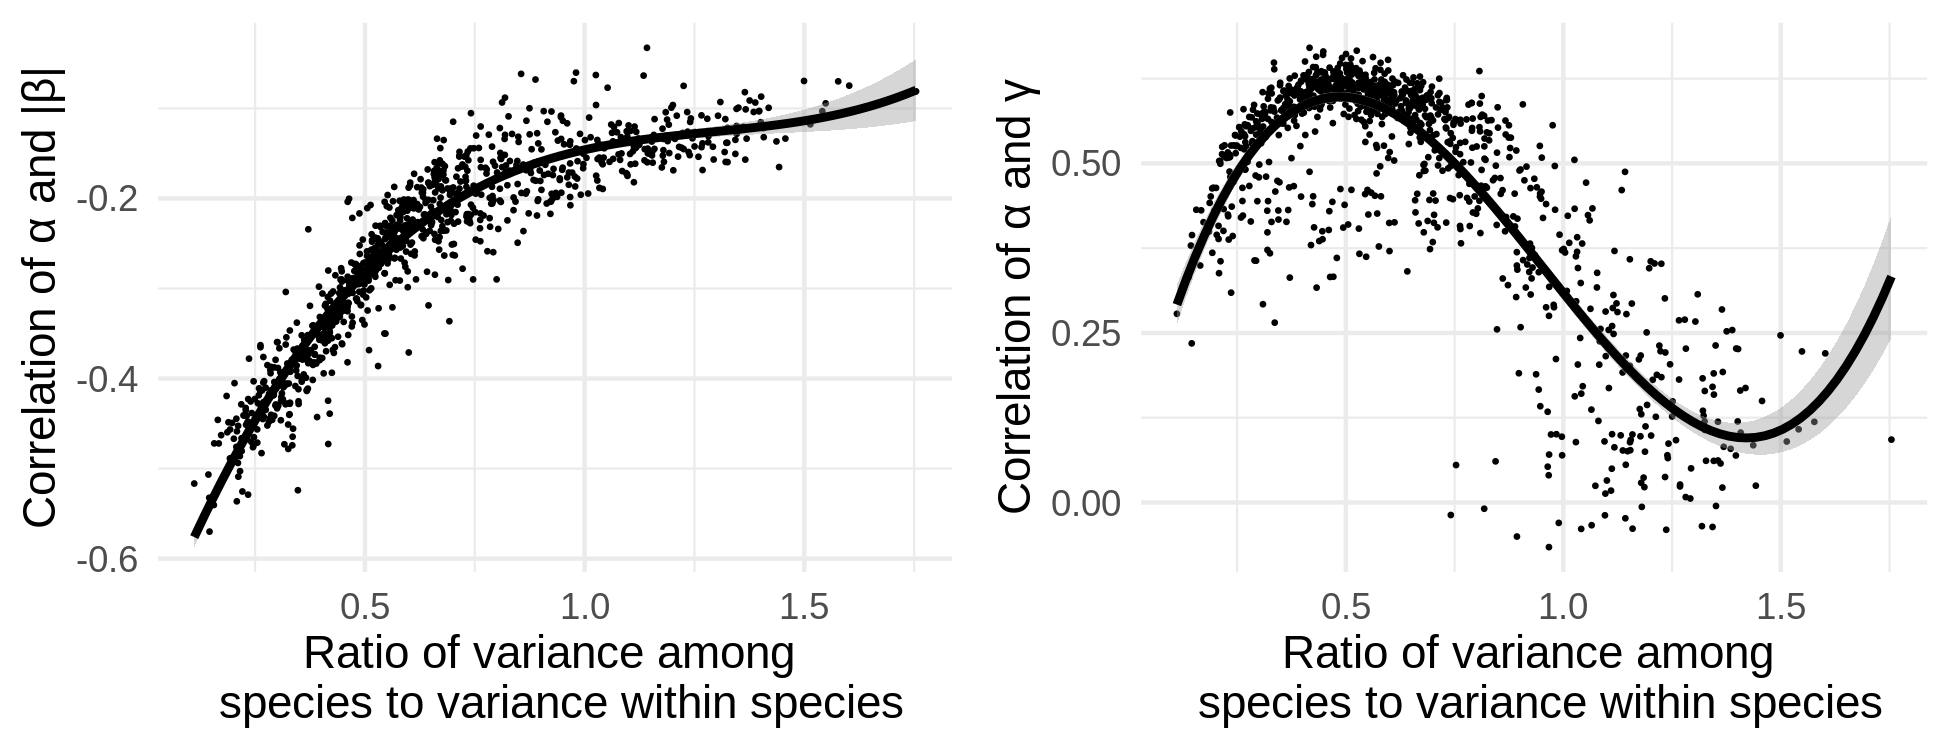
\includegraphics[width=1\linewidth,]{/home/bb/Gits/branching.brownian.motion.and.spde/Current Version/corrs} 

}

\caption{\label{num_corr} Numerical estimate for the correlations of selection gradients and competition coefficients.}\label{fig:unnamed-chunk-1}
\end{figure}

\newpage

\hypertarget{references}{%
\section*{References}\label{references}}
\addcontentsline{toc}{section}{References}

\hypertarget{refs}{}
\leavevmode\hypertarget{ref-Champagnat2006}{}%
Champagnat, Nicolas, Régis Ferrière, and Sylvie Méléard. 2006.
``Unifying Evolutionary Dynamics: From Individual Stochastic Processes
to Macroscopic Models.'' \emph{Theoretical Population Biology} 69 (3).
Elsevier BV: 297--321.

\leavevmode\hypertarget{ref-DaPrato2014}{}%
Da Prato, Giuseppe, and Jerzy Zabczyk. 2014. \emph{Stochastic Equations
in Infinite Dimensions}. Cambridge University Press.

\leavevmode\hypertarget{ref-lawrenceevans2010}{}%
Evans, Lawrence C. 2010. \emph{Partial Differential Equations: Second
Edition}. American Mathematical Society.

\leavevmode\hypertarget{ref-stanleyfarlow1993}{}%
Farlow, Stanley J. 1993. \emph{Partial Differential Equations for
Scientists and Engineers}. Dover.

\leavevmode\hypertarget{ref-meleard1992interacting}{}%
Méléard, M, and S Roelly. 1992. ``Interacting Branching Measure
Processes.'' \emph{Stochastic Partial Differential Equations and
Applications (G. Da Prato and L. Tubaro, Eds.)}, 246--56.

\leavevmode\hypertarget{ref-Mlard1993}{}%
---------. 1993. ``Interacting Measure Branching Processes. Some Bounds
for the Support.'' \emph{Stochastics and Stochastic Reports} 44 (1-2).
Informa UK Limited: 103--21.

\leavevmode\hypertarget{ref-zheng2004nonlinear}{}%
Zheng, Songmu. 2004. \emph{Nonlinear Evolution Equations}. Boca Raton,
Fla: Chapman \& Hall/CRC Press.

\end{document}
